\documentclass{article}

\usepackage[british,UKenglish,USenglish,english,american]{babel}
\usepackage[utf8]{inputenc}
\usepackage{amsmath}
\usepackage{amssymb}
\usepackage{anysize}
\usepackage{color}
\usepackage{xcolor}
\usepackage{graphicx}
\graphicspath{ {./images/} }
\usepackage{babel,blindtext}
\usepackage{hyperref} % % package for inserting Hyperlinks
\usepackage{tikz}
\usetikzlibrary{shapes,snakes}
\usetikzlibrary{shapes.misc, shapes.arrows}
\usetikzlibrary{calc, matrix,chains,scopes,positioning,arrows,fit}


\usepackage{listings}
\lstset{
	language=C++,                	% choose the language of the code
	basicstyle=\footnotesize,       % the size of the fonts that are used for the code
	numbers= left,                 	% where to put the line-numbers
	numberstyle=\footnotesize,      % the size of the fonts that are used for the line-numbers
	stepnumber=2,                   % the step between two line-numbers. If it is 1 each line will be numbered
	numbersep=5pt,                  % how far the line-numbers are from the code
	backgroundcolor=\color{white},  % choose the background color. You must add \usepackage{color}
	showspaces=false,               % show spaces adding particular underscores
	showstringspaces=false,         % underline spaces within strings
	showtabs=false,                 % show tabs within strings adding particular underscores
	frame=single,           		% adds a frame around the code
	tabsize=2,          			% sets default tabsize to 2 spaces
	captionpos=t,          			% sets the caption-position to bottom (t=top, b=bottom)
	breaklines=true,        		% sets automatic line breaking
	breakatwhitespace=false,    	% sets if automatic breaks should only happen at whitespace
	escapeinside={\%*}{*)}          % if you want to add a comment within your code
}

\usepackage{caption}
\usepackage{subcaption}
\DeclareCaptionFont{white}{\color{white}}
\DeclareCaptionFormat{listing}{\colorbox{gray}{\parbox[c]{\textwidth}{#1#2#3}}}
\captionsetup[lstlisting]{format=listing,labelfont=white,textfont=white}

\setlength\parindent{0pt}
\setlength{\parskip}{10pt}

\marginsize{3cm}{2cm}{2cm}{2cm}

\title{Software Engineering Project}
\author{Donatas Kozlovskis, Enric Cornellà\\
		Andrey Pak,  Fernando Garcia\\
		VIBOT-8}
\date{11/12/13}

\begin{document}
\maketitle

\section{Introduction}

The present document illustrates all decisions, procedures and methodology followed during the development of the application map. But also specific documentation regarding the implementation such as diagrams or remarkable algorithms specifically designed to solve the problems from the implementation.

This document has been divided in three different main sections; the first one shows the time line followed for carrying out the project and the common decision taken regarding the two other following sections, the second section focusses on the C++ implementation and finally, the last one, focusses on the Matlab part. 

\subsection{Tools and resources}
This section shows which software has been used directly or indirectly during the whole phase of design as well as the phase of development.
In order to manage the whole our project and its tasks, we have chosen the web-based project management application \textit{Trello}. It allows to keep track of everything, from the big picture to the minute details. In this way, all kind of tasks can be divided and assigned to the people involved in the project and also can be located in different boards according to the state of development of the task as in the following image:

\begin{figure}[!h]
\centering
\includegraphics[width=0.68\textwidth]{trello.png}
\caption{Image of the task manager during the development process at early stages. The work is divided in four different boards with multiple drag and drop tasks and is assigned to one person}
\end{figure}

At the same time, real world meetings were not avoided. Normally, we tried to establish team meeting at least once in a week. In such meetings we have discussed common problems, created good ideas or simply tried to brainstorm as many ideas as possible. Afterwards, the results of such meetings were definitely moved to the interactive board in \textit{Trello}.

\begin{figure}[!h]
\centering
\includegraphics[width=0.6\textwidth]{windowBoard.jpg}
\caption{One of the team meeting. Window is used as a white board to gather all ideas/problems.}
\end{figure}

Concurrently we were looking for frameworks for managing software projects. We have found that \textit{Agile software development} methods as \textit{Scrum} could fit to iterative management development of our project, however as it requires a lot of knowledge, we left this framework to the future works and employed only general parts of this framework.

For every developer's team, it is also important to establish the IDE and tools before starting to develop the project. On one hand, we assigned that \textit{open-source} Qt 5.0.1 OpenGL under Mingw compiler would be the appropriate platform because it is the last stable version of Qt and also because this open source developing environment allows us to create easier the graphical user interface and also render without adding by hard the OpenGL libraries. On the other hand, regarding to Matlab part, everything has been developed using the R2013a version of the software.

However, the previous software is not the only one used in the project. We supposed correctly the basic necessity to deal with data structures such as information related with roads, nodes, buildings or points of interest among other possible types (see section \textit{Methodology}). The options were to deal with this data coming from one, \textit{txt/xml} format files or similar or two, databases.
In both cases, Matlab and C++ implementation, the decision was to work with databases because of the amount of data and specially because is the easiest and fastest way to get detailed information of the structures without going over the whole structure in such cases as getting nodes shared by two different roads (see the \textit{Database} section).

Despite sharing the same EER schema, the database chosen for the Matlab part is different from the one chosen for the C++ part. In this way, we decided to use PostgreSQL just because it is easier to make it work together with Matlab and using MySQL 5.6 with Qt which was more familiar to us. But also, the fact that we chose two different databases made us able to change between them if some problems of generation had been encountered. Note that we have used the correspondent browsers for both platforms.

Finally, a source code management (SCM) system \textit{GIT} hosted in bitBucket (https://bitbucket.org) was used to control the different versions of the code and to be able to maintain work at the same time easily.

\subsection{Related works}

In order to be able to design a user-friendly and helpful application it is necessary to have a look to the current work, for instance GoogleMaps (https://maps.google.com/) or another non common but open-source solutions as MapGuide (http://mapguide.osgeo.org/) or OpenStreetMap (http://www.openstreetmap.org/). 

Checking the last solution we found the way to get most of the data required to render our map and to fulfil our databases. In addition, some of the information provided by this source was not used.

For user's information, \textit{OpenStreetMap} data is stored in topological data structure. Basically there are 4 data primitives as the basic components of \textit{OpenStreetMap}: nodes, ways, relations and tags. For us the first element was a main ingredient as geographical data source and the second element \textit{ways} represents relationship between various nodes. 

\textit{OpenStreetMap} has been a good provider of data but at the same time it has been necessary to adapt our database tables to the information obtained and in some cases to add some additional parameters because we have to take into account that this platform is not able to provide a route between two points, at least not in a direct way. For example, all elements as roads, forest, buildings, rivers, linear structures are represented as polygons of \textit{way} data primitives, thus additional data filtering, subsets were used to prepare required datasets for implementation of project database.

\clearpage
\section{Application Design}
In this section is explained how the application was devised starting by the definition of the database as well as the analysis of the use cases taking into account the user and the design of the resultant graphical user interface prototype.

\subsection{Use cases} \label{use_cases}
In order to prototype the graphical user interface of both parts, we conceived the diagram of cases of use that the user could find. But, first of all, which use cases we have?

According to the statement provided in requirements we can identify the following cases:

\begin{itemize}
  \item Finding the shortest path between two nodes picked up from the screen providing information about distance and time depending on the way of transport.
  \item Finding the shortest path between three points including the same information.
  \item Locating a point of interest.
  \item Finding all points of interest of a specific type around one place.
  \item Creating/Modifying/Deleting a point of interest.
\end{itemize}

That also can be summarized in the following diagram:

\begin{figure}[h]
\centering
\includegraphics[width=0.6\textwidth]{use_cases.png}
\caption{Diagram of the use cases provided to the user}
\end{figure}

The user has to be able to select a point of interest which already exists, modify it and deleted from the database. But also has to be able to create a new point of interest and simply locate it on the map.

Once the user selects a point from the map, no matters if it is random position or a point of interest, we have the option to establish the distance we want to locate a specific type of points of interest around it. But also, we have the option to select a second or still a third point of interest for getting the shortest path.

\subsection{GUI prototype}
After defining the use cases that users have to be able to deal with, we can start prototyping the graphical user interface that is also common between the two implementations. To accomplish this hard task that can be adjusted to solve future requirements, we decided to divide the screen in 5 different relevant points explained below:

THE BROWSER: This section is marked with the number one in the following figure, first GUI prototype. Basically, it brings to the user the possibility to look for a point of interest that is already present in the database.

THE MAP: The zone shows a map able to be scaled (zoom in and zoom out) and reactive to mouse events in the whole surface.

SHORTEST-PATH: Number Three allows the user to establish a route between two or three points taking into account if he or she is moving by car or by foot. But also brings the possibility using the buttons located on the left, to look for a type of point of interest around one position.

POINTS OF INTEREST: Both Buttons located in number four allows the user to create a new point of interest or modify an existing one through a form.

ROUTE: Finally, number five the distance and time that the user will spend having selected some locations previously. Showing the turns and the distances between them. Also brings the possibility to download all this text in a \textit{txt} file.

\begin{figure}[h]
\centering
\includegraphics[width=0.7\textwidth]{Prototype.png}
\caption{First GUI prototype conceived at early stages of the design process}
\label{fig:GUIprototype}
\end{figure}

\subsection{Getting the data}
With the aim of creating a robust database where solving the problems proposed by the statement and in order to the maintain the wholeness of the data inside we have to consider the following statement:

\textit{"One map is composed by ROADS which in turn are composed by different NODES. However, a node could belong to more than one road which identifies an intersection between two roads. The only attributes necessary for a node would be a unique ID and the position of the node in a map defined by LATITUDE and LONGITUDE. In the same way all roads have the following attributes: A unique ID that identifies it, its NAME, a TYPE that describes if the road can be used by cars and finally, if it can be passed in both WAYS."}

Here, we can identify two tables, its attributes and the relation between them which can be defined as N:M because of the fact that one node can belong to multiple roads, and one road can have multiple nodes. But also this relationship has to be defined taking into account the order the node has in the road that belongs to, giving an attribute of the relationship called ORDER.

On the other hand, the user has to be able to see the points of interest, create news, delete them and also modify the ones which already exist. We decided to create two tables in the same schema without any relationship with the previous tables in order to maintain the isolation from the points updated all the time because it does not belong to any specific road.
The number of attributes considered from the very beginning for the points of interest (POI) table are: The ID and the position in LATITUDE and LONGITUDE, the NAME of the point, as well as the ADDRESS and the TYPE. Taking into account the previous steps, we can see the result of the database in the following schema:

\begin{figure}[h]
\centering
\includegraphics[width=0.53\textwidth]{big_schneider.png}
\caption{Diagram of the relational database model created during the design}
\label{fig:RelDBdiagram}
\end{figure}

Notice that part of the process of development and parsing of the data from OpenStreetMap into our databases was accomplished together with the rest of the groups as well as the large amount of points of interest collected from Le Creusot. However, almost everything has been adapted to our specific requirements creating new tables, adding new columns and making homogeneous all information collected. 

\clearpage
\section{C++ Implementation}
The present section has been divided in two different parts: The first one explains how the map structure is created evolving the three basic classes, the correspondent adjacency matrix depending on the choice of the user (walking or driving), how the shortest path is calculated using Dijkstra's algorithm and the logic behind the management of the points of interest. During the second part, we will focus on how the data is shown and obtained directly from the screen and its process of normalization and denormalization, taking into account the different spatial coordinates we work with during the implementation. But also we will see how the graphical user interface provides the input/output to the user and how is managed.

\subsection{Creating the map}
The implementation of the application started with classes \textit{Node}, \textit{Road} and \textit{Map} according to the three tables already existing in the database and with the goal of loading all necessary points that composes the map of Le Creusot in memory. However, at the same time, we wanted to take profit of the whole process storing all nodes that composes one road in the same structure. As a consequence, the map structure is a vector container that keeps as many pointers to road structures as number of roads are in the map. At the same time, each road is a vector container whose size is defined by the number of nodes that compose it. However, what is stored in the road structure are pointers to nodes.

\begin{lstlisting}
vector<Road*> myMap 			//Definition of map structure
vector<Node*> myRoad;			//Definition of road structure
map<unsigned int,Node*> nodes;	//Definition of translator ID/Node
\end{lstlisting}

Trying to improve the performance, the class also has a structure used as a dictionary between the ID node and the node itself. Then, all searches have a complexity $ O(log(n)) $.

\begin{figure}[h]
\centering
\includegraphics[width=0.6\textwidth]{map.png}
\caption{UML diagram of the three classes that composes the logic map: Map, Road and Node}
\end{figure}

As we can see our class \textit{map} has dependencies with the class \textit{QtSQL}, necessary for making queries to the database but also contains a standard map structure. It is used in order to avoid checking node by node in some cases, a map that contains the node structures and its identifier is composed in the constructor. Finally, we can see some other dependences with standard libraries with \textit{QtOpenGL} the library that makes possible drawing the nodes that compose the map (explained in detail in the next section).

\subsection{The shortest path}
The first requirement from this kind of application is to be able to provide the shortest route between two specific nodes in the map. In order to carry on this task there are a lot of common and tested algorithms available such as Bellman-Ford, its variation called  Shortest Path Faster Algorithm (SPFA), Jonhson's algorithm, Floyd–Warshall algorithm, Dijkstra's algorithm.

Bellman-Ford algorithm and its variation is believed to work properly with graphs that contain negative weights as edges although for graphs without negative values, Dijkstra improves the performance. In the same direction both Jonhson's and Floyd-Warshall algorithms are more suitable for graphs which contain negative values in the their edges. Because of that, we finally decide to use a Dijkstra's algorithm.

Finally, the class has a method called \textit{calcTime()} which calculates the time spend if the user had did the route walking or driving considering the speed as 4km/h for people and an average of 40km/h for cars.

\subsubsection{Dijkstra's algorithm}
Despite the implementation of the algorithm is well known, we would explain slightly the basis using pseudo-code given a graph G, with edges E, vertices V and a source vertex s. We can define the following structures:

\begin{itemize}
  \item dist: Array of distances from the source to each vertex.
  \item prev: Array of pointers to preceding vertices.
  \item i: Loop index.
  \item F: List of finished vertices
  \item U: List or heap unfinished vertices
\end{itemize}


\begin{lstlisting}
/* Initialization: set every distance to INFINITY until we discover a path */
for i = 0 to |V| - 1
    dist[i] = INFINITY
    prev[i] = NULL
end

/* The distance from the source to the source is defined to be zero */
dist[s] = 0

/* This loop corresponds to sending out the explorers walking the paths, where
 * the step of picking "the vertex, v, with the shortest path to s" corresponds
 * to an explorer arriving at an unexplored vertex */

while(F is missing a vertex)
   pick the vertex, v, in U with the shortest path to s
   add v to F
   for each edge of v, (v1, v2)
        /* The next step is sometimes given the confusing name "relaxation"
        if(dist[v1] + length(v1, v2) < dist[v2])
            dist[v2] = dist[v1] + length(v1, v2)
            prev[v2] = v1
            possibly update U, depending on implementation
        end if
    end for
end while

//Extracted from: http://www.cprogramming.com/tutorial/computersciencetheory/dijkstra.html
\end{lstlisting}

\subsubsection{The adjacency matrix}
The following section describes a specific method of the \textit{map} class that allows us to create an adjacency matrix of dimensions NxN where N is the total amount of nodes that composes the map. This matrix will be used to calculate the shortest path between two or more points in the map. Such matrix is generated according to the method of transport chosen by the user. For instance, we can not drive in both senses in all roads or driving in a foot way.

First of all, the structure is allocated in memory and initialized to the maximum distance in all positions, in our case 0 units, and 0 in the diagonal of the squared matrix. Then, the rest of the matrix is filed taking into account the distance between the nodes identified by the index of the rows and columns of the matrix. From this point, the only thing we have to do is to go over the map structure checking which nodes are consecutive meaning that exists a connection between them. In this way, the position $M_{adj}(1,2)$ would contain the distance between node 1 and node 2. But what happens with the position $M_{adj}(2,1)$? This position contains the same distance if and only if the road is two ways, fact that can be checked querying the attribute \textit{oneWay} located in table \textit{Roads} in the database. 
We can also take into account querying the database, if a road is a foot way or not and calculate the appropriate distance.
On the other hand, people can work in both senses and also use all king of roads, so we can generate the adjacency matrix in the same way without the restrictions explained above. Notice that in order to calculate the distance between two nodes the method \textit{distNode()} was implemented in class \textit{node } following the formula of the euclidean distance. 
However, during the process of development the number of nodes was increased in order to test the real performance of the algorithm with a larger number. It highlight the weaknesses of performance generating and storing the adjacency matrix in memory. Let us see and example: 4 Bytes (float) * 84·$10^{6}$ (number of nodes) $\simeq$ 336 MB

In order to solve this issue and at the same time improving the access response to the elements, we decided to use sparse matrices to take out, somehow, all zeros that composes the adjacency matrix, reducing its size. For carrying out this task, we have used Eigen \footnote{Eigen is an open source C++ library of template headers for linear algebra, matrices, vectors and operations between them. See \url{ http://eigen.tuxfamily.org/index.php?title=Main_Page}} library. The main idea behind this is the compression of the data through the compressed sparse column (CCS) where the values are readed by column and a row index is stored for each one in a vector. Then, all non zero values are stored in an a new array. 

In addition, among the benefits already explained, we can also see how the performance of the Dijkstra's algorithm improves according to the size of the matrix in the following table \footnote{All this results have been measured in Debug mode and also depends completely on the performance of each processor speed}:

\begin{table}[ht] 
\caption{Sum up of the benefits of Sparse matrices}
\centering
\begin{tabular}{c c c}
\hline\hline 
~ & Matrix & Sparse \\ [0.5ex]  
\hline 
Num. nodes & $\simeq$84·$10^{6}$ & $\simeq$16·$10^{3}$ \\
Memory & $\simeq$336 MB & $\simeq$64 KB + Zero vector\\ 
Time & $>$30 sec & $<$1 sec \\ 
Dijkstra &  $>$30 sec & $<$3 sec \\ [1ex]
\hline
\end{tabular} 
\label{table:nonlin}
\end{table} 

\subsection{Route path}
The current functionality is compressed in the \textit{patch} class and allows the user to see the way which has to follow to perform the shortest path between the points already selected.
The main working principle is based on the angle defined by groups of three nodes. Let us consider a specific clarifier example where the nodes provided by the shortest path algorithm are in red. If the i-2 and i nodes belongs to the Road 2 we know we are just going straight ahead. However, when we consider if the nodes i-1 and i+1 belongs to the Road 2, we can notice that they are not meaning that we turned right or left. Then, we can calculate the angle of the three points and obtain a value around 90 degrees if we are turning right according to the point of view of the user. Or conversely, if we obtain an angle around -90 means that we are turning left.

Now, we can imagine a lot of exceptions derived from the general case as when the same street changes its name or when we find a intersection of more than 2 roads involved on it. In the first case, the algorithm takes into account that the angle is still around 180. And in the second one, we can stablish some borders where we can show messages such as: "turn slightly...".

Finally, all these orders can be exported to a \textit{txt} file using \textit{genTxt()} method of the class.

\begin{figure}[h]
\centering
\includegraphics[width=0.3\textwidth]{angle.png}
\caption{Example of road cross in the calculation of the route path}
\end{figure}

\subsection{Points of interest}
Regarding to the points of interest, our first decision was to keep them in the database because of the large list we had collected (around 200 points of interest of more than 20 types). However, this table has no relationship with table \textit{node} because, in general, all points have a specific location that does not correspond to any node in the map: Maybe because of the real latitude and longitude setted manually using a GPS or maybe because of the point pressed on the screen does not correspond to any node.

In this way, we can print all points of interest in their specific location in the map, over buildings, parks... away from roads but at the same time keeping the independence with the table \textit{node}. Then, when the user wants two calculate the shortest path to a point of interest, the route brings him to the closest node that composes the map. Otherwise, we should generate an adjacency matrix including all points of interest when a new point is created taking an overhead of memory.

The different types of points of interest are composed in the following: Bakery, Bank, Bar/Restaurant, Cars, Church/Cemetery, Cigar Store, Cultural place, Florist, Fuel, Grocery, Hairdressing, Hospital, Hotel, Park/Library, Pharmacy, Post Office, Residence, School, Shop, Sports/Gym, Train Station, University Building and Variety store.

\subsection{Graphical user interface}
The graphical user interface of the C++ implementation has been one of the challenges of this project: it had to control the large amount of different relationships and dependencies with another already existing files and our goal to take control of all possible situations and exceptions generated by the user performing any actions. We solved those situations using resources such as disabling buttons or showing pop-up messages when the user chooses an invalid option. In the next sections, explanations of such solutions and implementation of the requirements specified in section \ref{use_cases} are given.

\subsubsection{Heuristics}

Since we are not avoiding self-criticism, we could mention that the user interface created is not a best one and it would be useful to look at it from the point of view of heuristic evaluation. Heuristics were taken from the list released by Jakob Nielsen in 1994.

\begin{itemize}

	\item \textbf{Visibility of system status: }
	The user interface generally follows this heuristic, however there are some violations. The computation of the route using Dijkstra algorithm is relatively long and there is no status bar responsible for displaying the progress of the route computation. On each route computation time, the program windows freezes for a certain period of time (1-3 seconds) which is not comfortable to the user.
	
	\item \textbf{Match between the System and the Real World: }
	The System should speak the Real World's language. This heuristics is partially violated in the route display algorithm. When the users selects a route from the screen, the text explanation displayed doesn't contain the names of the roads  (implementation issue). The only information showed is the distance and direction of where to move. From the user point of view it would be confusing.
	
	\item \textbf{User control and freedom: } 
	The most of the actions performed by the user can be easily reverted. When the user picks a point from the map, he or she can easily remove it by clicking the corresponding "cross" on the left side of the screen. (It would have been also useful to decrease the distance of the mouse movements by introducing this option in the right-click context menu, but it was avoided due to the lack of the developer's experience.)
	When adding or modifying the Point of Interest, a "Cancel" or "Reset" buttons revert the changes that were not committed yet.
	This heuristics is violated in the "Delete" action of the POI management window. The system doesn't request a confirmation and just displays the window with the information that the POI was successfully deleted.
	
	\item \textbf{Error prevention: }
	The error prevention is realized by enabling the elements of the GUI only when they require user's attention and disabling them otherwise. For example, when browsing through the existing POIs, all edit fields are disabled, however, when switching to edit mode, all browsing widgets are disabled and edit fields are enabled. Also, when the "Custom" POI type is set in the point of the main screen, it is impossible to choose any known point of interest.
	A small tip is provided in the left bottom corner of the main screen regarding some special aspects of the program.
	
	\item \textbf{Flexibility and the efficiency of use: }
	There couldn't be a lot of keyboard shortcuts in this kind of program. Only About (F1) and Quit (Ctrl+Q).
	
	\item \textbf{Aesthetic and Minimalist design: }
	Not aesthetics, but functionality was in priority when developing the GUI. The majority of the screen is occupied by the map widget and the rest of the screen doesn't contain any unnecessary controls.
	
	\item \textbf{Help User Recognize, Diagnose and Recover from Errors: }
	This is not a big program, so the amount of possible errors is small. The majority of the errors come from the database interaction and route computation. The errors are followed by the pop-up messages that try to explain the origin of the error (not always).
	
	\item \textbf{Help and documentation: }
	As mentioned before, the "About" action exist, but it doesn't provide a lot of information. Some tips are displayed on the main screen.
	Developer documentation was generated by Doxygen.
	
\end{itemize}

\subsubsection{Normalization and displaying}

One of the main problems encountered was the conversion between geographic, OpenGL and widget coordinates. Those three systems use different references, e.g. in our program node coordinates are expressed using latitude and longitude while the OpenGL widget requires pixel coordinates from the center of the screen, so it is necessary to perform the conversion each time we use them.

When converting the coordinates from geographic to OpenGL, the problem is quite straightforward and it is a simple mapping problem.

So, we have to map a coordinate ranging from $x_{min}$ to $x_{max}$ to the coordinates ranging from $y_{min}$ to $y_{max}$. We can consider it as a linear equation:

\begin{equation}
y = ax + b
\end{equation}

So, we have two equations:
$$
\begin{cases}
y_{max} = ax_{max} + b \\
y_{min} = ax_{min} + b
\end{cases}
$$

From this equation we receive a and b:

\begin{equation}
a = \frac{y_{max} - y_{min}}{x_{max} - x_{min}}
\end{equation}

\begin{equation}
b = -a\frac{x_{max} - x_{min}}{2}
\end{equation}

So, when normalizing the coordinates we just calculate a and b and perform the computation. It is also necessary to note that geographic coordinates are stored in the latitude - longitude manner, so we have to inverse these coordinates while painting it inside the OpenGL.

In our case, we normalize these values to the size of the texture mapped inside the OpenGL. Another problem arose from the OpenGL requirements where the dimensions of the texture should be the powers of two (2048 x 1024 .png image in our case). So, after exporting an image of the texture from the OpenStreetMap we have to crop it and calculate the approximate values of the latitude and longitude which results in the loss of precision.

However, when trying to get the geographic coordinates of the point where user clicked, we have to consider the ratio between the size of the QGLWidget and the size of the OpenGL's viewport inside it and the map movement. In addition to that, first we should transform the point from widget to OpenGL coordiantes, then to geographic coordinates.

The final algorithm for getting the geographic coordinates out of widget coordinates when the ration between the viewport and the widget is one (so, one pixel in OpenGl corresponds to one pixel in the widget), is as follows:

First, we calculate the position of the cursor in OpenGL by translating the widget coordinates with zero in the top left corner of the screen to the standard 2D cartesian plane of the OpenGL.

\begin{lstlisting}
    float mpoglx = (widgetCoordinates.x() - width()/2) - movPos.x();
    float mpogly = -(widgetCoordinates.y() - height()/2) - movPos.y();
\end{lstlisting}

Then, we calculate a (2) and b (3) and perform the inverse transformation with some modifications:

\begin{lstlisting}
    float mpgeolon = (mpoglx*0.5/scale - bLon)/aLon;
    float mpgeolat = (mpogly*2/scale - bLat)/aLat;
\end{lstlisting}

???



-Explain process of normalization and denormalization.
-Classes used using inheritance such as QGLWidget, UI or QmainWindow
-Geo to OpenGL Coordinates and find closest

\subsubsection{Selecting a route}
In order to make the route selection as user friendly as possible, we have created a main menu which is able to perform all tasks related with routes divided in five parts (see figure~\ref{fig:menu_poi}): Method of transport, type of point of interest in the second column, specific point of interest in the first column, deletion and points of interest management (explained in detail in section \ref{POI}).

Fist of all, the user has to select the way of transport using the radio button. Once it is selected, whatever point of the map can be pressed as initial point "Custom" or by contrast, a point of interest can be selected in the first column sorting by type in the second one and finally, be setted as initial point. We also can do exactly the same with a target point, selecting from the map or from the list filtering by type. Moreover, we could select a third point in the same way and define a shortest path between an initial and end point, and a target in the middle. For sure, whatever of the three points could be deleted from the path maintaining the rest of the route unbroken.

However, we have to take into account that for finding the path to, for instance, the closest bakery, it does it calculating first the euclidean distance between all bakeries and then doing Dijkstra to the closest one. This is because the cost to perform the shortest path to all bakeries and compare the distance is computationally really expensive despite the fact that is easy to code.

In this way, we can get the distance of the whole path as well as the route path for the user in order to reach the different targets and also export this route as a \textit{txt} file.

\begin{figure}[h]
\centering
\includegraphics[width=0.5\textwidth]{menu_points.png}
\caption{Menu displayed for performing the shortest-path between two or more points in the map or points of interest from the database taking into account the method of transport defined. The second column sorts by type, the first one selects the specific point of interest and the third one deletes the piece of path selected.}
\label{fig:menu_poi}
\end{figure}

\subsubsection{Points of interest management} \label{POI}
The most simple thing we can do regarding to the points of interest is to show them according to the type they belong to as we could see in figure~\ref{fig:menu_poi}: We can select the type in the box "display all". In addition, the points of interest basically has three different functions that are: Searching for specific point, modifying an already existing point of interest or creating a new one. For the first two options we can press directly the button "Manage POIs" that will open a form sheet (see figure~\ref{fig:sub1} ), where we can obtain different information such as address, coordinates, name and in some cases an image of the place. It is important to notice that since we are looking for information all fields are shown disabled. However, it the radio button is changed to "Edit" we could modify some parameters related with the place as is shown in image~\ref{fig:sub2}: Name, address, type of point of interest or image. As a final option, the point can be deleted using the correspondent button or execute the query for the data base saving the changes.

\begin{figure}[h]
\centering
\begin{subfigure}{0.5\textwidth}
  \centering
  \includegraphics[width=.8\linewidth]{form.png}
  \caption{Searching mode}
  \label{fig:sub1}
\end{subfigure}%
\begin{subfigure}{0.5\textwidth}
  \centering
  \includegraphics[width=.8\linewidth]{form1.png}
  \caption{Editing mode}
  \label{fig:sub2}
\end{subfigure}
\caption{The different options can be available or not depending on the Browse or edit function in the radio button}
\label{fig:test}
\end{figure}

Since no coordinates has been selected form the map, if has pressed the radio button "New" nothing would have happened, showing a pop-up to the user suggesting to press a point from the screen. Then, the way to have access to create a new point of interest is to press first a point on the screen. Basically, the image showed remains the same but with empty fields and taking care of fill all parameters

\clearpage
\section{Matlab Implementation}
       
In this section the project implementation using Matlab is discussed and presented. Most of the concepts are reused from C++ source code as the preservation of consistency between two different sources was one of the our purposes. Thus here, the text will focus the reader only on the differences between concepts and code.

\subsection{Getting the data}

As it was mentioned before, in Matlab implementation we have chosen to use \textit{PostgreSQL} database, since the whole process (installing additional drivers for Matlab, making connectors, etc.) was more user friendly and time efficient. However, the database schema/structure and all data were the same between MySQL and PostgreSQL implementations (see figure: ~\ref{fig:RelDBdiagram}).

The first difference comes in fact that the \textit{variables} in Matlab can be not even created, but as well saved in and loaded from Matlab's data structure \textit{.mat} files. This allowed us to come to the solution where the connection to external data source (database) is made only one time for creating appropriate data structures/class objects (discussed in next section). As in Matlab project part queries to database are used only one, the program end-user does not need to have database and driver installed, because afterwards all calculations are created using generated data structures from .mat files.

\subsection{Data Structure}

The second important question which had to be answered - the types of data structures in Matlab.
Since by itself Matlab has a lot of different data types from which the \textit{struct} objects can be created, we have decided to create our  own object \textit{classes} with required properties and methods. The reader should note, that there a lot of differences between Matlab and other OOP languages, all of those will not be discussed since all information can be found in the web.\footnote{
\url{http://www.mathworks.fr/fr/help/matlab/matlab_oop/matlab-vs-other-oo-languages.html}
}

Another faced issue was the fact that the Matlab is not so flexible as C++ with passing objects by pointer or reference. Since we would like to avoid creating a copies of original objects in functions, we found that \textit{handle} classes in Matlab can be created, where class constructor returns a handle object that by itselfs is a reference to the object created. In this way, using such objects in functions, MATLAB copies just the handle and access its data indirectly.

As in C++ implementation, classes for representing the \textit{node}, \textit{road} and \textit{map} were created.

\begin{figure}[!h]
\centering
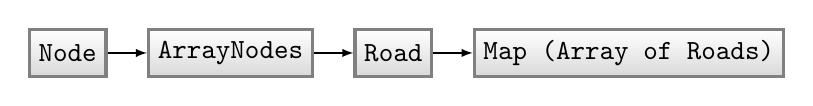
\begin{tikzpicture}[node distance=5mm,
terminal/.style={
% The shape:
rectangle,
minimum size=6mm,
% The rest
very thick,draw=black!50,
top color=white,bottom color=black!15,
font=\ttfamily}]

\node (Node) [terminal] {Node};
\node (ArrNode) [terminal,right=of Node] {ArrayNodes};
\node (Road) [terminal,right=of ArrNode] {Road};
\node (Map) [terminal,right=of Road] {Map (Array of Roads)};
\path
(Node) edge[-latex] (ArrNode) % simple edges
(ArrNode) edge[-latex] (Road)
(Road) edge[-latex] (Map);

\end{tikzpicture}
\caption{Simplified diagram of relationship of a classes}
\end{figure}

As opposite to C++ implementation, here the additional class \textit{ArrayNodes} was created. This was done with intention to vectorize some methods, since Matlab is optimized for operations involving matrices and vectors. Of course, it was possible to implement such methods directly to the road class, though the recent approach was chosen to emphasize that methods are only related with the Array of \textit{Nodes}.

Notwithstanding our option, the user could find an alternative or better data structure for the same goal.
For example, together with the team we discussed another options such as keeping data for our project in the same way as in kept in the database: roads and nodes tables and the dictionary (linking table) between roads and nodes. Such structure would have it's advantage that various connections between roads and nodes would be easier accessible, e.g. it would be possible to get all roads where node \textit{X} is included and vice versa, while the our methodology requires additional methods to get the same results. 

% % matlab
% % Shortest Path
\subsection{The shortest path}
This issue was common between both versions (C++ and Matlab) of programs, thus the same algorithms were used to get a solution to the question of shortest path (Dijkstra was employed on a weighted graph represented as adjacency (sparse) matrix). Therefore in this section the user's attention will be focused on a question how to find a shortest path starting from a random Map Point, which is not pre-included in a adjacency matrix.\\
Firstly, the random point needs to be obtained from the map with relevant Longitude/Latitude coordinates. The second step is to answer the question, how should we include this new point into already existing weighted graph? After discussion with team members, we came up to the solution where the new point should be connected with a closest existing node. However, there could be a case where the already existing node is closest to the new point, but another perpendicular projection to the line segment, represented using two other nodes is shorter then the distance between new point and already found closest node. Thus, finally we decided employ both methods. Please note, that the latter method (projection) requires adding two new points to the weighted graph and the weights between user input - projected point, projected point and two nodes of line segment should be added as well.
Basically, all algorithm can be summarized in such steps:
\begin{itemize}
\item Determine the window on which the closest nodes and projections will be searched.
\item Find the closest node on determined window.
\item Find the closest projection (if possible) on the same window.
\item Update the adjacency matrix according shortest distance.
\end{itemize}

 

% % % % % % % % % % % % % % % % % % % % % % % % % % % % % % %
% projection figure
\begin{figure}[!h]
\centering
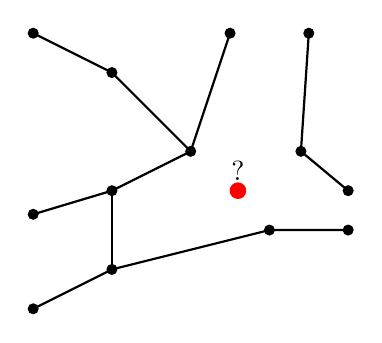
\begin{tikzpicture}[
	%	style def
    scale=1,
    important line/.style={thick},
    every node/.style={color=black}
    ]
	
	% demo connection of nodes
	\draw[important line] (0,1) coordinate (a1) -- (1,1.5) coordinate (a2) -- (3,2) coordinate (a3) -- (4,2) coordinate (a4);
	\draw[important line] (0,2.2)coordinate (C2) -- (1,2.5) coordinate (D) -- (2,3) coordinate (E) -- (2.5, 4.5) coordinate (F);
	\draw[important line] (a2)--(D) ;
	\draw[important line] (E)--(1,4) coordinate (G) -- (0,4.5) coordinate (H);
    \draw[important line] (3.5,4.5)coordinate (I) -- (3.4,3) coordinate (J)  --  (4,2.5) coordinate (K) ;
    \fill[black] 
        		 (a1) circle (2pt)
    			 (a2) circle (2pt)
    			 (a3) circle (2pt)
    			 (a4) circle (2pt)
    			 (C2) circle (2pt)
    			 (D) circle (2pt)
    			 (E) circle (2pt)
    			 (F) circle (2pt)
    			 (G) circle (2pt)
    			 (H) circle (2pt)
    			 (I) circle (2pt)
    			 (J) circle (2pt)
    			 (K) circle (2pt);
    %circle representing user input			 
    \fill[red] (2.6,2.5) circle (3pt) node[above] {$?$};
\end{tikzpicture}
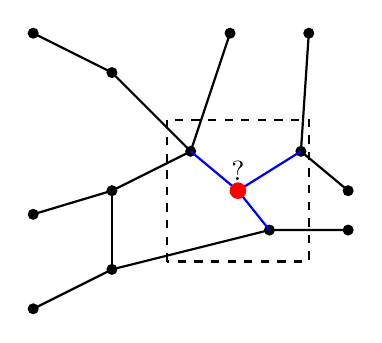
\begin{tikzpicture}[
	%	style def
    scale=1,
    important line/.style={thick},
    every node/.style={color=black}
    ]
	
	% demo connection of nodes
	\draw[important line] (0,1) coordinate (a1) -- (1,1.5) coordinate (a2) -- (3,2) coordinate (a3) -- (4,2) coordinate (a4);
	\draw[important line] (0,2.2)coordinate (C2) -- (1,2.5) coordinate (D) -- (2,3) coordinate (E) -- (2.5, 4.5) coordinate (F);
	\draw[important line] (a2)--(D) ;
	\draw[important line] (E)--(1,4) coordinate (G) -- (0,4.5) coordinate (H);
    \draw[important line] (3.5,4.5)coordinate (I) -- (3.4,3) coordinate (J)  --  (4,2.5) coordinate (K) ;
    \fill[black] 
        		 (a1) circle (2pt)
    			 (a2) circle (2pt)
    			 (a3) circle (2pt)
    			 (a4) circle (2pt)
    			 (C2) circle (2pt)
    			 (D) circle (2pt)
    			 (E) circle (2pt)
    			 (F) circle (2pt)
    			 (G) circle (2pt)
    			 (H) circle (2pt)
    			 (I) circle (2pt)
    			 (J) circle (2pt)
    			 (K) circle (2pt);
    %circle representing user input			 
    \fill[red] (2.6,2.5) coordinate(user) circle (2pt) ;
    			     

    \draw[important line, blue] (user) -- (a3);
    \draw[important line, blue] (user) -- (E);
    \draw[important line, blue] (user) -- (J);
    %connecting closest nodes
        %circle representing user input			 
        \fill[red] (user) circle (3pt) node[above] {$?$};
        
    %square window line (dashed)
    \draw[important line, black, dashed] (2.6-0.9,2.5-0.9) -- (2.6-0.9,2.5+0.9) -- (2.6+0.9,2.5+0.9) -- (2.6+0.9,2.5-0.9) -- (2.6-0.9,2.5-0.9);
    
\end{tikzpicture}
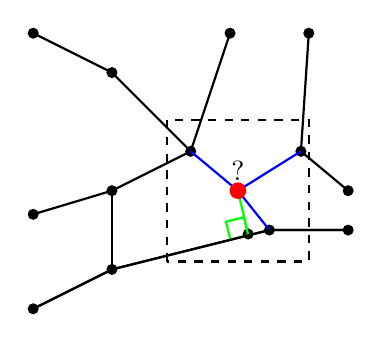
\begin{tikzpicture}[
	%	style def
    scale=1,
    important line/.style={thick},
    every node/.style={color=black}
    ]
	
	% demo connection of nodes
	\draw[important line] (0,1) coordinate (a1) -- (1,1.5) coordinate (a2) -- (3,2) coordinate (a3) -- (4,2) coordinate (a4);
	\draw[important line] (0,2.2)coordinate (C2) -- (1,2.5) coordinate (D) -- (2,3) coordinate (E) -- (2.5, 4.5) coordinate (F);
	\draw[important line] (a2)--(D) ;
	\draw[important line] (E)--(1,4) coordinate (G) -- (0,4.5) coordinate (H);
    \draw[important line] (3.5,4.5)coordinate (I) -- (3.4,3) coordinate (J)  --  (4,2.5) coordinate (K) ;
    \fill[black] 
        		 (a1) circle (2pt)
    			 (a2) circle (2pt)
    			 (a3) circle (2pt)
    			 (a4) circle (2pt)
    			 (C2) circle (2pt)
    			 (D) circle (2pt)
    			 (E) circle (2pt)
    			 (F) circle (2pt)
    			 (G) circle (2pt)
    			 (H) circle (2pt)
    			 (I) circle (2pt)
    			 (J) circle (2pt)
    			 (K) circle (2pt);
   %circle representing user input			 
    \fill[red] (2.6,2.5) coordinate(user) circle (2pt) ;
    			     
	%connecting closest nodes
    \draw[important line, blue] (user) -- (a3);
    \draw[important line, blue] (user) -- (E);
    \draw[important line, blue] (user) -- (J);
    % projection
    \draw[important line, green] (user) -- (2.73, 1.95) coordinate (intersect);
    \fill[black] (intersect) circle (2pt) ;
    
    \draw[important line, green, ] (intersect)+(-0.14,0.07) node[minimum size=0.1cm,draw,green, rotate =14]{};
    %circle representing user input			 
    \fill[red] (user) circle (3pt) node[above] {$?$};
    \draw[important line] (a1) -- (a2) -- (a3) -- (a4);   
    
    %square window line (dashed)
    \draw[important line, black, dashed] (2.6-0.9,2.5-0.9) -- (2.6-0.9,2.5+0.9) -- (2.6+0.9,2.5+0.9) -- (2.6+0.9,2.5-0.9) -- (2.6-0.9,2.5-0.9);	 
\end{tikzpicture}
\caption{Finding the shortest point/projection for the random point on window domain}
\end{figure}

\subsection{Graphical User Interface (GUI)}

The \textit{Graphical User Interface} is one of the most important parts of every program nowadays. The user requires a simple way to interact with the software and the GUI provides it. We came up with a simple idea shown in Figure \ref{fig:GUIprototype}, and after a few updates and modifications we got the next one:

\begin{figure}[h]
\centering
\includegraphics[width=0.8\textwidth]{gui.png}
\caption{Graphical User Interface designed in Matlab}
\label{fig:guiMatlab}
\end{figure}

As we can see it is divided into 5 parts. In the next points we will explain briefly what each part does and after we will discuss it thoroughly.

\begin{enumerate}
\item
In this first part we will be able to modify the points represented on the map. As we can see we will have three different options in order to choose a point:
	\begin{itemize}
	\item
	Choose an element from the whole list.
	\item
	Filter the points by class, for example to show only the restaurants.
	\item
	Choose a random point by clicking on the map.
	\end{itemize}
We have \textit{Point 1} and \textit{Point 2}, which will be the basic points.

\item
In the second part of the GUI we can decide if we want to go by foot or by car. This parameter will affect the button \textit{GO!} that will compute the shortest path between the two selected points.

\item
In this third part we can observe four different buttons: \textit{POI, Itinerary, Find in a Range} and \textit{Instructions}. This will change the panel shown in the point 4.

\item
In this part we will change the panels according to the button we pushed. At the beginning the POI menu is visible but the user can interact with anyone.

\item
The last one, the number five, is the map. Here is where we will plot all the results computed in the background operations.
\end{enumerate}

In the next subsections we will explain in detail how every part of the GUI works and how it interacts with the background functions.

\subsubsection{Introduction of points by the user}
Selecting two points and going from the first to the second is probably the most basic thing one would expect from this kind of application. That's why we made it simple and easy to access. As shown in the previous figure for every point we will be able to choose three different methods. 

The \textbf{first} one and very simple is to choose a point from a list. At the beginning we load all the Points Of Interest (POIs) from a .mat file. All this POIs were extracted from a common work between all the groups and contain a great amount of interesting places of Le Creusot. We do a little filter in order to choose only the name of the places since this file contains other information. Then the user selects a point by scrolling and clicking or by typing in the keyboard and pressing enter. When a point is selected the program follows the next steps:

\begin{itemize}
\item
First of all the callback of the function is called.
\item
Then we extract the index number and we will use it to know which POI has been selected. We do this by using the next function:
	\begin{lstlisting}
	contents = get(hObject,'Value');
	\end{lstlisting}
The \textit{contents} variable will be a number.
\item
We initialize two arrays containing the latitudes and longitudes of the actual POIs list, by the moment all of them. Then we extract the latitude and longitude of the point selected by accessing at the posicion \textit{contents} of these variables. Note that in this point we will store the variables in the handles since we want this point to be accessible from another part of the program and not only this callback.
\item
The next thing to do is to check if we have any Point1 displayed, if this is the case we delete it. Then it is plotted in the map so the user can easily see it. Note that the points will appear according to the colour used in the background of the selection menu of each point. The points are plotted also in a handle so it can be deleted in anywhere without deleting the background map.
\item
Finally we actualize the handles.
\end{itemize} 

The \textbf{second} way to introduce a point allows the filtering by classes. It is very similar to the first one but it adds extra possibilities to the common way. It is easier and faster to find points.

To do this the user must select one of the classes introduced in the program. When it is selected we go into a function that will filter the main data file into a smaller one. This function compares the class of each POI and if it matches with the selected one it adds the information of this point to a new variable. To compare the two strings we use \textit{strcmp()}, used in the C++ labs. This will create a new list with only one class POI information. When going back to the main GUI program we will store this list into the actual POI data and we will update the information in the main pop-up menu. In this way when the user will see only the selected class points in the pop-up menu.

In this part we faced some problems when selecting first a POI by the first method and the filtering by classes. After a few hours we saw the error was caused by the index of the menu. If we selected first the POI number 35 and then we filtered by a class that only contains 6 elements it crashed. This is because it was trying to access the 35th position of the new list and it didn't exist. The way to solve this problem was to reset this value to 1 so whenever the user changes anything the pop-up menu it is updated to the first position automatically.

The \textbf{third} method had a very simple implementation. By clicking on the button \textit{Get Loc.} the user is able to point anywhere in the map and select a point, that is stored in the handles of longitude and latitude. The function used is \textit{ginput(1)}, very common in Matlab. The we plot the point in the map the same way we did in the other two methods.

\subsubsection{Selecting how to reach the point and calculating the shortest path}

In this second part we will explain how the selection of going by foot or by car is done and also how the shortest path will be computed.

Starting by the beginning, we can see in point two of the GUI image the user is able to select going by car or by foot. This will affect the way we call the functions in the background when selecting \textit{GO!}. Depending on which one is selected we will pass the handle of the sparse matrix \textbf{Car} or the sparse matrix of \textbf{Walk}. The function \textit{twoInputShortestPath} will compute the shortest path and return it together with the distance. Right now we can ignore the last parameter since we don't need it.

When we get the shortest path we plot it so the user can see in the map the way to follow. It will also generate a set of instructions, but this will be explained in a few pages.

Finally we have to take in care the case the user entered wrongly some points or he left one by mistake. If this occurs we have designed a special window that will appear showing an error message. In order to avoid the creation of multiple windows for different errors that we may encounter, this little GUI will show the message passed by the main program. So in this case we will have something like this:

\begin{lstlisting}
GUI_error('One or more points are invalid, please recheck it');
\end{lstlisting}

\subsubsection{Menus for interaction}

In this subsection we will be explaining how the menus works and which are the possibilities for the user to interact. This part concerns the points 3 and 4 of the image since they are strongly linked.

The \textbf{POI} menu has two main functionalities: manipulation of the \textit{Points of Interest} and the \textit{Refresh} button. The POIs can be modified or created depending on the needing of the user. In the two cases a new user interface will appear. In the case of modifying a POI in the first thing to do is to choose an existing point. In this moment all the data of this point is charged in the window and the user can see it. The user changes the wrong information to update it and then saves it. At this point the .mat file containing the data of all POIs is updated and there is no way back to restore this file.

The same happens with the creation of a new POI. The user is asked to insert all the data needed. Here we are not controlling all the data fields are filled, so you can save an empty point or with invalid data. In addition the user cannot create a new class of points of interest.

In th next figure we can see the two windows and how are organized:

\begin{figure}[h]
        \centering
        \begin{subfigure}[b]{0.3\textwidth}
                \includegraphics[width=\textwidth]{modify_poi}
                \caption{Modify a POI}
                \label{fig:modify_poi}
        \end{subfigure}%
        \qquad %add desired spacing between images, e. g. ~, \quad, \qquad etc.
          %(or a blank line to force the subfigure onto a new line)
        \begin{subfigure}[b]{0.3\textwidth}
                \includegraphics[width=\textwidth]{new_poi}
                \caption{Set new POI}
                \label{fig:new_poi}
        \end{subfigure}
        \caption{Manipulation of Points of Interest}\label{fig:manipulation_poi}
\end{figure}

The \textbf{Refresh} button is quite useful in this application. Since the user will be computing multiple paths or itineraries it will be necessary to clean the plots of the screen and to reset the variables (classes, POIs, etc.). The implementation is very easy since the only things to do will be: resetting the pop-up menus in order to look like in the opening of the program, check if there are some plots to delete and set all the handles of the points to 0. Despite some of this functions are implemented in buttons such as \textit{GO!} it is recommended to do a refresh every time we want to compute a new path so we will avoid to have corrupted data if we forget to change some parameters or points.

The \textbf{Itinerary} button will allow the user to choose a middle point when calculating the path. For example we can go from Carrefour to IUT passing by a bakery and we want the path to be shorter than XXXX meters. Let's see how the menu itinerary looks when pressing the button:

\begin{figure}[h]
\centering
\includegraphics[width=0.3\textwidth]{itinerary}
\caption{Itinerary menu}
\label{fig:itinerary}
\end{figure}

As you can see we are able now to set 3 POIs in the map. Note that automatically the button GO has disappeared since a new one is placed in the menu. This is done because here we will need to calculate the shortest path two times in order to show it. Basically the working principle is the same as the simple GO but now duplicating the work since we have 3 points.

Unlike when we are working only with two points we need now the distance of the two paths in order to compare it with the one inserted by the user. If the distance is greater than the requested one we display an error message using the previously created error GUI, otherwise we display the path and create the instructions.

The part of the itinerary takes approximately twice of time than the two points shortest path. So the user will have to wait for a few seconds while the program is computing it.

When we press the third button \textbf{Find in range} a new menu appears. This allows the user to find places near one point. Since it will look for classes of points of interest this will become very useful. It makes it really easy to find bakeries for example. Let's see how this new menu looks like.

\begin{figure}[h]
\centering
\includegraphics[width=0.3\textwidth]{find_range}
\caption{Find in range menu}
\label{fig:find_range}
\end{figure}

As we can see the first thing to do is to determine the position of the user in order to start looking for POIs. To do this we ask the user to interact with \textit{Point 1} so we can avoid creating a new insertion of POIs. Once the user has defined this position we ask for the class of point to find. Here appears a pop-up menu updated with all the classes and the user selects one of them. Finally introduces the maximum distance from the point and the program will compute the result when pressing the button \textit{FIND!}. Once computed it will display the points in the map and we will use again the error GUI but this time not for showing any error. The name of the POIs found will be shown in this window. 

Parameters such this maximum distance are stored in handle variables initialized in the beginning of the program. When the user inserts a value the callback of this function is called automatically and the value is stored. This makes the work easier since we don't need to be checking every time these values, they are updated when the user changes the value.
 
Finally in this set of menus we have the option \textbf{Instructions} which as the name indicates it will show how to reach our destination. In the main GUI, when we have computed the shortest path, we simply call this function and it will return some text in a very long string. In order to read it we add the word 'NewLine' every time it should break and the we split it using \textit{strsplit}. This will create a cell array and in each cell we will have a sentence of this instructions. Using the function set we will insert this text in \textit{Edit Text} box where we have setted the \textit{Enable} property to \textit{inactive} so you cannot modify anything inside this box. Here we also added a scrollbar in the right side because sometimes the instructions are very long and they don't fit in the size of the text box.

In the next figure we can observe an example of the instructions window with some text inside.

\begin{figure}[h]
\centering
\includegraphics[width=0.3\textwidth]{instructions}
\caption{Instructions menu}
\label{fig:instructions}
\end{figure}
 
As we can see we go down with the scrollbar and finally at the end there exists the possibility to export the data in a .txt file. This will create a file in the directory where the program is executed with the name \textit{instructions.txt}. Note that this file will be overwritten every time we generate a new instruction set so if you want to save it you have to change the name of it.

As the data was collected by all the groups and jointed together some roads are missing and sometimes we can find unnamed streets in the instructions. This can be solved by manually finishing the own database of points of interest.

\subsubsection{Plotting the map}

Finishing the menus we only have one thing left and it is the \textbf{map plotting}. This is done initially in the beginning of the program when the opening function of the GUI is executed. We call the plotMap function that is executed in two parts. First of all to understand how will it work we should think in a plot painted by layers where we can remove or add parts to show. First of all we should start filling the plot by the last layer, the one that we will always to be visible and this one is the image of the map, to give a view like the classical \textit{Google Maps}. Secondly we will plot all the roads in an upper layer so we can see both of them (map and roads). Up to this part we can consider it the static part of the map. Then during the execution of the program, as we have already explained, we will plot some points and lines in an upper layer that can be removed.

See the next figure to try to understand how it works.

\begin{figure}[h]
\centering
\includegraphics[width=0.3\textwidth]{map_plot}
\caption{Map}
\label{fig:map_plot}
\end{figure}

In this figure we use up to 4 layers to plot. From lower to higher are:
\begin{enumerate}
\item
Background image.
\item
All the roads.
\item
Points of interest.
\item
Shortest path (in red).
\end{enumerate}

If you take a look again in the map plot you will be able to see the roads represented in different colours and width. This is a visual way to recognise the bigger streets and also the paths only for pedestrians only.

\subsubsection{Organization of the data}

In this subsection we will explain a little bit how the data is structured inside the main GUI program and how it works. One of our great friends in this part has been the \textbf{Handles}. This is a structure containing handles to all the objects created in the graphical user interface so we can manipulate everything from any point of the code. This has been very useful for storing data such the latitudes and longitudes of the actual points or the different variables that will determine if a point is plotted or not.

One important thing about the handles is they need to be updated whenever we change the value of them, otherwise they will not update. This was a minor problem at the beginning when learning how it worked the callbacks and GUIs of Matlab since sometimes we forgot to update the handles and the results were not the expected ones.

When calling the function \textit{twoInputShortestPath} we cannot give the handles to it. Instead we must create a \textit{mapNodeStart} and a \textit{mapNodeTarget} points, which belongs to a class. This is the way the background functions work, with classes.

The files of data are stored in \textit{dependencies\textbackslash data}. The two important ones for the GUI are \textit{POIdata.mat} and \textit{POIClasses.mat}. The first one is a file that contains all the points of interest gathered by all the groups. We needed some filtering of this data before storing it here since some data was wrong. The file is a matrix of cells and it contains as many rows as POIs has and 5 columns. In these we can find the latitude, longitude, name, class and address of each POI.

We access this cells in different parts of the program depending on which data do we need. When we create a new class filter we preserve this 5 columns but we only select a few POIs. Then we store it directly in the handles instead of saving it in a file.

\clearpage
\section{Conclusion}
During all development process we have seen how Matlab is more suitable for performing tasks of prototyping, it is easy and fast to develop with and also brings to the user a countless number of resources such as algorithms to deal with the shortest path, it is already optimized regarding to the manipulation of matrices and large amount of data structures and brings the possibility to build easily graphical user interfaces.

On the other hand, using C++ we can obtain a finished product that when it is executed performs much more better in real time even it is more tedious during the development process. We can see this evidence for instance, when we try to compute Dijkstra's algorithm in real time in both implementations and how fast behaves in the C++ implementation in comparison with Matlab code. 

Despite the all differences of C++ and Matlab environments, we have tried to preserve consistency between two different sources. However, some methodologies which work fast in one environment are not so effective in other, (e.g. looping in Matlab, or passing data by pointers is not possible directly in Matlab), thus the user can see the different codes and algorithms on two programming languages. Also, the Matlab program is dependent on IDE version installed to machine, which limits the user to have portable version of a program, which could be made easily using C++ release.

We have seen in Matlab how easy is to create a GUI, however this has a little cost. The possibilities of making element different are not very high. Matlab provides a closed environment for working in the graphical interfaces where it is very easy to do a button or to put some text but it is quite closed to customize them. In C++ it is harder to program an interface but the options are bigger since the limitations of programming are less. This is an extra point for Matlab if we don't need really good GUIs but a point for C++ if we need a good finishing touch.


\clearpage
\section{Appendix}

- Documentation, resources and additional files can be found at (check Readme.txt file): 

\url{https://www.dropbox.com/sh/9ci2o6xctwog3kf/JM1tnjTTxT}

- Full source code with history, changes, all works can be found at SCM server online:

\url{https://bitbucket.org/DonatasKozlovskis/seproject} 

- We can show some of the more important functions and their relationships in the following diagrams regarding to the C++ implementation:

\begin{figure}[h]
\centering
\includegraphics[width=0.7\textwidth]{2.png}
\caption{Whatever change in the list of points of interest as well as the events in the map screen generates a recalculation of the route path shown.}
\end{figure}

\begin{figure}[h]
\centering
\includegraphics[width=0.8\textwidth]{4.png}
\caption{When we add a point, the coordinates of this one has to be normalized to be displayed in the map because the range is too small for OpenGL. In addtion, if the point is created pressing the screen, it has to be linked to a node using 'findClosest' to be able to calculate the paths. For doing that, we perform Dijkstra's algorithm generating an 'output' and printing it (\textit{PrintPath()}) with the estimation time (\textit{CalcTime}). Then , we are ready to calculate the instructions checking the angles between the nodes and the distance between them.}
\end{figure}

\begin{figure}[h]
\centering
\includegraphics[width=0.8\textwidth]{6.png}
\caption{When MapGLWidget is generated the first time, we query the data base to compose the map and normalize the values and according to these points, the adjacency matrix is composed using the 'disNode' function.}
\end{figure}

\begin{figure}[h]
\centering
\includegraphics[width=0.6\textwidth]{8.png}
\caption{When a point of interest is modified using the correspondent form, the following methods are used to set the new parameters}
\end{figure}

\begin{figure}[h]
\centering
\includegraphics[width=0.8\textwidth]{9.png}
\caption{The diagram shows the times that a query to the data base is executed: Firstly, when we load initially the data structure in the MapGLWidget. Secondly, when we have to add, delete or modify a point of interest. And finally, when we display the points of interest filtering by type.}
\end{figure}

\end{document}